\section{Programmation}

\subsection{Programmation orientée objet (POO)}

Nous avons fait le choix d'utiliser une fonctionnalité très utile du langage C++, la programmation orientée objet. La programmation orientée objet (POO) est un moyen de concevoir et de construire des programmes informatiques en utilisant des \emph{objets}.

Chaque objet a des caractéristiques, telles que l'apparence ou les fonctionnalités, qui sont décrites dans un plan appelé \emph{classe}. La classe définit comment l'objet doit se comporter et quoi faire lorsqu'on lui envoie des messages ou des instructions.

L'objectif de la POO est de modéliser le monde réel en utilisant des objets qui représentent des entités réelles, telles que des personnes, des voitures ou des robots. Les objets peuvent interagir les uns avec les autres en envoyant des messages et en appelant des \emph{méthodes}.

La POO est largement utilisée dans la programmation moderne et est prise en charge par de nombreux langages de programmation, tels que Java, Python, C++ et bien d'autres. En utilisant la POO, les développeurs peuvent créer des programmes plus robustes, plus flexibles et plus faciles à maintenir.

\noindent Dans le cas de notre projet, nous avons un objet \emph{Robot}, nommé \textbf{\textit{goofyBot}} tout au long du projet, initialisé avec des valeurs du constructeur :

\begin{lstlisting}[language={C++}, caption={Fichier robot.hpp contenant la classe Robot}, label={robot.hpp}]
#ifndef ROBOT_HPP
#define ROBOT_HPP

#include <mbed.h>

class Robot {

public:
    Robot();

    DigitalOut IHM_Led1;
    DigitalOut IHM_Led2;
    DigitalOut IHM_Led3;
    DigitalOut IHM_Led4;

    DigitalIn IHM_Btn1;
    DigitalIn IHM_Btn2;
    DigitalIn IHM_Btn3;
    DigitalIn IHM_Btn4;

    DigitalIn jack;
    DigitalIn finCourse;
    AnalogIn mesureBatterie;
    AnalogIn captLigneDroiteInt;
    AnalogIn captLigneDroiteExt;
    AnalogIn captLigneGaucheInt;
    AnalogIn captLigneGaucheExt;

    PwmOut moteurDroit;
    PwmOut moteurGauche;
    DigitalOut moteurDroitSens;
    DigitalOut moteurGaucheSens;

    int jackVal;
    int fcVal;
    double mbVal;
    double dIntVal;
    double dExtVal;
    double gIntVal;
    double gExtVal;

    /** Fonction de debug du robot
     *  Affiche les valeurs des capteurs sur le port série.
     * 
     *  @note Teste les capteurs de ligne, de fin de course, de batterie et le jack et 
     *  démarre en même temps le mode débug de l'IHM.
     * 
     *  @warning Le robot doit être connecté à un ordinateur pour afficher les valeurs sur le port série.
     */
    void debugMode();

    /** Déplace le robot en fonction des PWMs des moteurs gauche et droit et des sens des moteurs
     *
     *  @param pwmGauche Valeur du PWM du moteur gauche entre -100 et 100 (reverse et forward)
     *  @param pwmDroit Valeur du PWM du moteur droit entre -100 et 100 (reverse et forward)
     */
    void move(float pwmGauche, float pwmDroit);
};

#endif

\end{lstlisting}

\begin{lstlisting}[language={C++}, caption={Constructeur de la classe Robot}, label={robot.cpp}]
// Constructeur
Robot::Robot() :
    // Assignation des pins
    jack(PTE20),
    finCourse(PTE21),
    mesureBatterie(A0),
    captLigneDroiteInt(A1),
    captLigneDroiteExt(A2),
    captLigneGaucheInt(A4),
    captLigneGaucheExt(A3),

    IHM_Led1(D15),
    IHM_Led2(D14),
    IHM_Led3(D13),
    IHM_Led4(D12),
    IHM_Btn1(D4),
    IHM_Btn2(D5),
    IHM_Btn3(A5),
    IHM_Btn4(PTE30),

    moteurDroit(D6),
    moteurGauche(D8),
    moteurDroitSens(D7),
    moteurGaucheSens(D9)
{ 
    // Initialisation des moteurs
    moteurDroitSens = 1;
    moteurGaucheSens = 1;
}

\end{lstlisting}

\subsection{Contrôler le robot}

Afin de faire fonctionner les moteurs grâce à la carte hacheur, nous avons une fonction appelée \emph{move} qui permet de contrôler le mouvement des moteurs du robot. Elle fait partie de la classe "Robot" et est donc accessible à tous les objets de ce type.

La fonction prend en entrée deux variables "pwmGauche" et "pwmDroit", qui représentent les niveaux de puissance pour les moteurs gauche et droit respectivement. La valeur de ces variables peut varier de -100 à 100. Si la valeur est positive, le moteur tourne dans un sens (sens avant), et si la valeur est négative, il tourne dans l'autre sens (sens arrière). Si la valeur est nulle, le moteur est arrêté.

La fonction définit tout d'abord la période pour les moteurs gauche et droit. Ensuite, le code effectue un certain nombre de calculs pour déterminer le sens de rotation du moteur et le niveau de puissance pour chaque moteur en fonction de la valeur d'entrée.

En somme, cette fonction permet de contrôler les moteurs du robot en fonction des entrées fournies, ce qui peut être utilisé pour contrôler le mouvement du robot dans différentes directions.

\begin{lstlisting}[language={C++}, caption={Fonction move()}, label={robot.cpp}]
void Robot::move(float pwmGauche, float pwmDroit) {
    // On définit la période des moteurs
    moteurDroit.period(T);
    moteurGauche.period(T);

    if(pwmGauche >= -100.0 && pwmGauche < 0) {
        moteurGaucheSens = 0; // Sens arrière
        pwmGauche = pwmGauche * -1.0;
        pwmGauche = pwmGauche / 100.0; // On divise par 100 pour avoir un pwm entre 0 et 1
    } else if (pwmGauche <= 100 && pwmGauche > 0) {
        moteurGaucheSens = 1; // Sens avant
        pwmGauche -= 100.0;
        pwmGauche = pwmGauche * -1.0;
        pwmGauche = pwmGauche / 100.0;
    } else if (pwmGauche == 0) {
        moteurGaucheSens = 1;
        pwmGauche = 1; // Stop
    }

    if(pwmDroit >= -100.0 && pwmDroit < 0) {
        moteurDroitSens = 0; // Sens arrière
        pwmDroit = pwmDroit * -1.0; // On inverse le signe du pwm
        pwmDroit = pwmDroit / 100.0; // On divise par 100 pour avoir un pwm entre 0 et 1
        //printf("%f", pwmDroit);
    } else if (pwmDroit <= 100 && pwmDroit > 0) {
        moteurDroitSens = 1; // Sens avant
        pwmDroit = pwmDroit - 100.0; 
        pwmDroit = pwmDroit * -1.0;
        pwmDroit = pwmDroit / 100.0; // On divise par 100 pour avoir un pwm entre 0 et 1
    } else if (pwmDroit == 0) {
        moteurDroitSens = 1;
        pwmDroit = 1; // Stop
    }

    // On applique le pwm aux moteurs
    moteurDroit.pulsewidth(T * pwmDroit);
    moteurGauche.pulsewidth(T * pwmGauche);
}

\end{lstlisting}

\subsection{Programmes}

La partie programmation du robot est séparée en trois fonctions principales du robot : deux fonctions permettant l'homologation du robot (Confettis et Carré) et la fonction suivi de ligne.

\subsubsection{Les confettis}

\begin{figure}[H]
\centering
\begin{minipage}{.5\textwidth}
  \centering
  \centerline{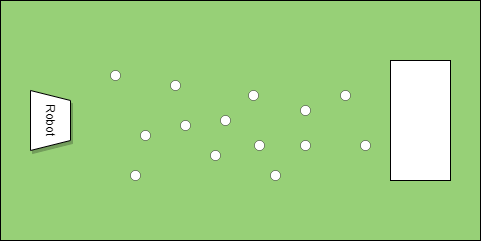
\includegraphics[width=1\linewidth]{img/parcours/confettie.png}}
  \captionof{figure}{\emph{Le robot doit passer par un chemin parsemé de confettis.}}
  \label{fig:confettis}
\end{minipage}%
\end{figure}

\vfill
\noindent\makebox[\linewidth]{\rule{.8\paperwidth}{.6pt}}\\[0.2cm]
I.U.T. Nice Côte d'Azur - SAE Robot - 2023 \hfill goofyBot
\noindent\makebox[\linewidth]{\rule{.8\paperwidth}{.6pt}}
\newpage

Cette fonction, nommée "confettis", utilise la bibliothèque "mbed" et la classe "Robot" définie dans "robot.hpp". Elle implémente un programme pour faire bouger un robot suiveur de ligne.

La fonction utilise une boucle infinie (while (1)) pour continuer à faire bouger le robot. A chaque tour de boucle, les entrées du robot (état de la valeur des capteurs de ligne) sont actualisées.

Ensuite, deux \emph{switchs} sont utilisés pour déterminer l'état du robot en fonction des entrées. Le premier switch détermine l'état suivant du robot en fonction de ses entrées actuelles, et le second switch détermine les actions à prendre pour chaque état. (cf. Machine à états)

\begin{figure}[H]
\centering
\begin{minipage}{.5\textwidth}
  \centering
  \centerline{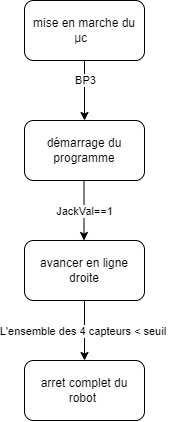
\includegraphics[width=0.5\linewidth]{img/mae/confettis.png}}
  \captionof{figure}{\emph{Machine à états : Confettis}}
  \label{fig:maeconfettis}
\end{minipage}%
\end{figure}

Par exemple, si le Jack est retiré (\emph{goofyBot.jackVal == 1}), l'état du robot passe à 2 et le robot bouge en avant (goofyBot.move(50,50)). Si les quatre capteurs de ligne détectent la ligne blanche (\emph{goofyBot.dIntVal <= 0.5 \&\& goofyBot.dExtVal <= 0.5 \&\& goofyBot.gIntVal <= 0.5 \&\& goofyBot.gExtVal <= 0.5}), alors l'état du robot passe à 4 et le robot attend pendant 25 000 microsecondes puis s'arrête (\emph{goofyBot.move(0,0)}).

\begin{lstlisting}[language={C++}, caption={Fonction confettis()}, label={confettis.cpp}]
void confettis(Robot& goofyBot) {
    int etat = 1;
    
    while (1) {
        goofyBot.jackVal = goofyBot.jack.read();
        goofyBot.dIntVal = goofyBot.captLigneDroiteInt.read() * 3.3;
        goofyBot.dExtVal = goofyBot.captLigneDroiteExt.read() * 3.3;
        goofyBot.gIntVal = goofyBot.captLigneGaucheInt.read() * 3.3;
        goofyBot.gExtVal = goofyBot.captLigneGaucheExt.read() * 3.3;

        switch(etat) {
            case 1:
                if (goofyBot.jackVal == 1) {
                    etat = 2;
                }
                break;
            
            case 2:
                if(goofyBot.dIntVal <= 0.5 && goofyBot.dExtVal <= 0.5 && goofyBot.gIntVal <= 0.5 && goofyBot.gExtVal <= 0.5) {
                    etat = 4;
                }
                break;
        }

        switch(etat) {
            case 2 :
                goofyBot.move(50,50);
                break;

            case 4 :
                wait_us(25000);
                goofyBot.move(0,0);
                break;
        }
    }
}
\end{lstlisting}

\subsubsection{Le carré}

\begin{figure}[H]
\centering
\begin{minipage}{.5\textwidth}
  \centering
  \centerline{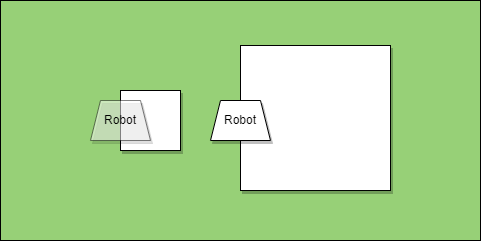
\includegraphics[width=1\linewidth]{img/parcours/carre.png}}
  \captionof{figure}{\emph{Le robot doit réaliser un carré.}}
  \label{fig:carre}
\end{minipage}%
\end{figure}

Ce code définit une fonction \emph{carre} qui fait que le robot exécute une forme carrée. La longueur du carré est déterminée par l'utilisateur via la fonction \emph{ihmSel()}. Le code utilise la méthode \emph{move()} de l'objet Robot pour contrôler le mouvement du robot. 

\vfill
\noindent\makebox[\linewidth]{\rule{.8\paperwidth}{.6pt}}\\[0.2cm]
I.U.T. Nice Côte d'Azur - SAE Robot - 2023 \hfill goofyBot
\noindent\makebox[\linewidth]{\rule{.8\paperwidth}{.6pt}}
\newpage

La fonction carré fait d'abord avancer le robot à vitesse constante sur une distance définie, puis fait tourner le robot en augmentant et en diminuant la vitesse des deux roues à des vitesses différentes. Le processus est répété 4 fois pour former une forme carrée.

\begin{figure}[H]
\centering
\begin{minipage}{.5\textwidth}
  \centering
  \centerline{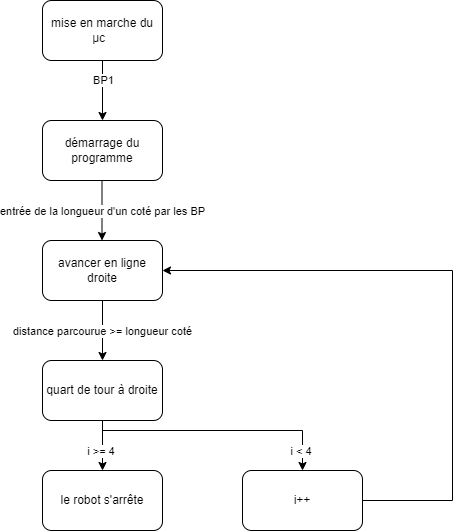
\includegraphics[width=1\linewidth]{img/mae/carre.png}}
  \captionof{figure}{\emph{Machine à états : Carré}}
  \label{fig:maecarre}
\end{minipage}%
\end{figure}

\begin{lstlisting}[language={C++}, caption={Fonction carre()}, label={carre.cpp}]
void carre(Robot& goofyBot) {
    int longueur = ihmSel(goofyBot);

    for(int i = 0; i < 4; i++) {
        goofyBot.move(45,45);
        wait_us ((longueur / 45.5) * 1000000) ;
        goofyBot.move(0,0);
        wait_us(500000);
        // augmentation et diminution progressive de la vitesse
        for(float speed = 25; speed < 90; speed += 5) {
            goofyBot.move(speed, -70);
            wait_us(14000);
        }
        for(float speed = 100; speed > 90; speed -= 5) {
            goofyBot.move(speed, -70);
            wait_us(14000);
        }
    }

    goofyBot.move(0,0);
}
\end{lstlisting}

\vfill
\noindent\makebox[\linewidth]{\rule{.8\paperwidth}{.6pt}}\\[0.2cm]
I.U.T. Nice Côte d'Azur - SAE Robot - 2023 \hfill goofyBot
\noindent\makebox[\linewidth]{\rule{.8\paperwidth}{.6pt}}
\newpage

Comme décrit ci-dessus, le côté du carré réalisé devra être compris entre 60cm et 200cm (2m). Pour cela, nous avons implémenté la fonction \emph{ihmSel()}. Celle-ci utilise l'intégralité de la carte IHM pour fonctionner. En effet, nous avons deux boutons de choix de taille (+10cm et +100cm) et deux boutons de validation (Reset et Valider).

\begin{lstlisting}[language={C++}, caption={Fonction ihmSel()}, label={ihm.cpp}]
int ihmSel(Robot& goofyBot) {
    // Taille en CM du carré (entre 60 et 200)
    int res = 0;
    while(goofyBot.IHM_Btn4.read() == 0) {
        goofyBot.IHM_Led2.write(0);
        if (goofyBot.IHM_Btn1.read() == 1) {
            // Ajout dizaines
            res += 10;
            wait_us(1000000);
        }
        else if (goofyBot.IHM_Btn2.read() == 1) {
            // Ajout centaines
            res += 100;
            wait_us(1000000);

        }
        else if (goofyBot.IHM_Btn3.read() == 1) {
            // Reset
            res = 0;
            wait_us(1000000);
        }
        
    }
    if(res > 200 || res < 60) {
        res = 0;
        for(int i = 0; i < 5; i++) {
            goofyBot.IHM_Led4.write(0);
            wait_us(100000);
            goofyBot.IHM_Led4.write(1);
            wait_us(100000);
        }
    }

    goofyBot.IHM_Led2.write(1);

    for(int i = 0; i < 5; i++) {
        goofyBot.IHM_Led1.write(0);
        wait_us(500000);
        goofyBot.IHM_Led1.write(1);
        wait_us(500000);
    }

    goofyBot.IHM_Led2.write(0);

    return res;
}
\end{lstlisting}

\vfill
\noindent\makebox[\linewidth]{\rule{.8\paperwidth}{.6pt}}\\[0.2cm]
I.U.T. Nice Côte d'Azur - SAE Robot - 2023 \hfill goofyBot
\noindent\makebox[\linewidth]{\rule{.8\paperwidth}{.6pt}}
\newpage

\subsubsection{Le suivi de ligne}

Et enfin, la dernière fonction et la plus importante, le suivi de ligne.

\begin{figure}[H]
\centering
\begin{minipage}{.5\textwidth}
  \centering
  \centerline{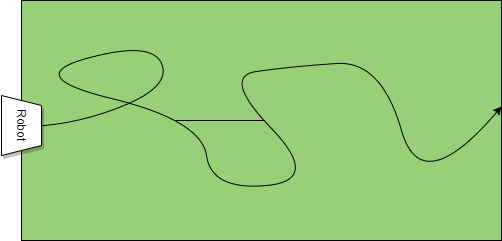
\includegraphics[width=1\linewidth]{img/parcours/suivideligne.png}}
  \captionof{figure}{\emph{Le robot doit suivre la ligne.}}
  \label{fig:suiviligne}
\end{minipage}%
\end{figure}

Afin de pouvoir allier vitesse et précision, nous avons décidé d'intégrer l'algorithme PID (\emph{Proportional-Integral-Derivative}), qui est un algorithme de contrôle utilisé pour maintenir une quantité mesurée, telle que la position, la vitesse ou la température, à une valeur souhaitée. Il est souvent utilisé  en automatisme et notamment dans la robotique pour contrôler les moteurs d'un robot ou d'un drone afin de maintenir une position ou une vitesse cible.   

L'algorithme PID utilise trois termes pour calculer le signal de commande pour les moteurs :

Proportionnel (P) : Le terme proportionnel est basé sur l'erreur actuelle entre la valeur mesurée et la valeur cible. Plus l'erreur est grande, plus le signal de commande sera fort.

Intégral (I) : Le terme intégral prend en compte l'accumulation de l'erreur au fil du temps. Cela peut aider à éliminer les erreurs à long terme et à améliorer la stabilité du système. (non utilisé ici)

Dérivative (D) : Le terme dérivatif est basé sur la vitesse de changement de l'erreur. Il peut aider à améliorer la réactivité du système et à éviter les oscillations.Plus il est élevé plus on tendra rapidement a la valeur de stabilité.

Les trois termes sont combinés pour produire le signal de commande pour les moteurs. Les constantes \textit{Kp}, \textit{Ki} et \textit{Kd} sont les gains PID qui peuvent être ajustés pour optimiser les performances du système de contrôle. Ils entrent aussi en équation avec la vitesse qu'il faut aussi régler avec précision pour obtenir un suivi de ligne optimal alliant fiabilité et rapidité.

\vfill
\noindent\makebox[\linewidth]{\rule{.8\paperwidth}{.6pt}}\\[0.2cm]
I.U.T. Nice Côte d'Azur - SAE Robot - 2023 \hfill goofyBot
\noindent\makebox[\linewidth]{\rule{.8\paperwidth}{.6pt}}
\newpage

\begin{figure}[H]
\centering
\begin{minipage}{.5\textwidth}
  \centering
  \centerline{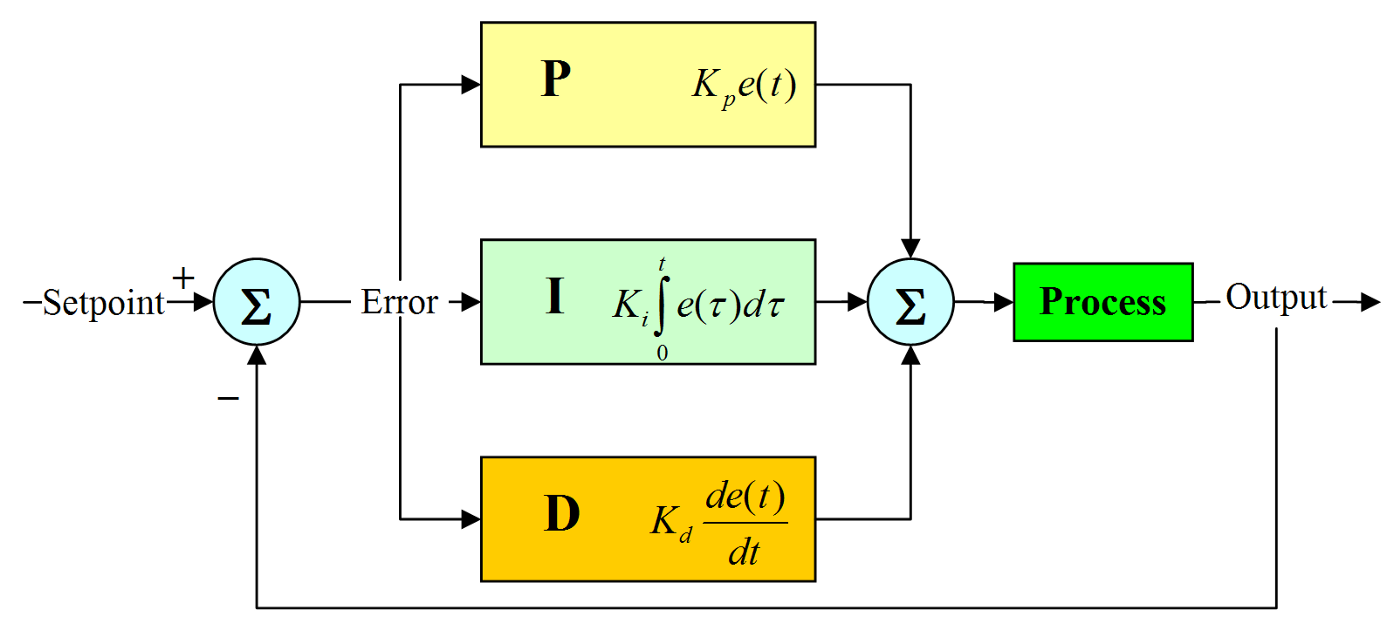
\includegraphics[width=1.2\linewidth]{img/pid.png}}
  \captionof{figure}{\emph{Schéma de l'algorithme PID.}}
  \label{fig:PID}
\end{minipage}%
\end{figure}

\begin{center}
    $u(t) = Kp * e(t) + Ki * \int_{0}^{t} e(\tau) \,d\tau + Kd \frac{de}{dt}(t)$
    
    Formule de l'algorithme PID prenant en compte les coefficients \emph{Kp, Kd et Ki}
\end{center}

\begin{lstlisting}[language={C++}, caption={Fonction suivi()}, label={suivi.cpp}]
#define SPEED 75
#define KP 45
#define KD 55

void suivi(Robot& goofyBot) {

    int etat = 0;
    float error = 0;
    float last_error = 0;
    float integral = 0;
    float derivative = 0;
    float PID_value, e, errorD, errorG;

    while(true) {
        goofyBot.jackVal = goofyBot.jack.read();
        goofyBot.fcVal = goofyBot.finCourse.read();
        goofyBot.dIntVal = goofyBot.captLigneDroiteInt.read();
        goofyBot.dExtVal = goofyBot.captLigneDroiteExt.read()*3.3;
        goofyBot.gIntVal = goofyBot.captLigneGaucheInt.read();
        goofyBot.gExtVal = goofyBot.captLigneGaucheExt.read()*3.3;
    
        e = ((goofyBot.gIntVal*3.3) - (goofyBot.dIntVal*3.3));

        error = (goofyBot.gIntVal - goofyBot.dIntVal);

        errorD = (goofyBot.dExtVal - goofyBot.gIntVal);
        errorG = (goofyBot.gExtVal - goofyBot.dIntVal);

        derivative = error - last_error;
        last_error = error;
        PID_value = (KP*error) + (KD*derivative);
        
        if(goofyBot.fcVal == 0) {
            etat = 69;
        }

        switch(etat) {
            case 0:
                if(goofyBot.jackVal == 1) {
                    etat = 1; //suivi
                } 
                break;
            
            case 1:
                if(e >= -0.05 || e <= 0.05) {
                    etat = 2;
                }
                break;

            case 2:
                if(goofyBot.dExtVal < 1.5 || goofyBot.gExtVal < 1.5) { //case extreme
                    etat = 3;
                }
                if (e >= 0.10 && e <= -0.10) {
                    etat = 1;
                }
                break;

            case 3: 
                if (e <= 0.02 && e >= -0.02) {
                    etat = 1;
                }
                if(e <= -0.10 && e >= 0.10) {
                    etat = 2;
                }
                break;
        }

        switch(etat) {
            case 0:
                if(e <= 0.03 && e >= -0.03) {
                    goofyBot.IHM_Led3.write(1);    
                } else {
                    goofyBot.IHM_Led3.write(0);
                }
                goofyBot.move(0,0);
                break;

            case 1:
                goofyBot.move(50,50);
                break;

            case 2:
                goofyBot.move(SPEED + PID_value, SPEED - PID_value);
                break;

            case 3:
                if(goofyBot.dExtVal < 0.7 || e >= 0.85) {
                    PID_value = (KP*errorD) + (KD*derivative);
                    goofyBot.move(SPEED + 10 + PID_value,0);
                }
                if(goofyBot.gExtVal < 0.7 || e >= 0.85) {
                    PID_value = (KP*errorG) + (KD*derivative);
                    goofyBot.move(0, SPEED + 10 + PID_value);
                }
                break;

            case 69: 
                goofyBot.move(0,0);
                break;
            }
        wait_us(5000);
    }
}
\end{lstlisting}

\vfill
\noindent\makebox[\linewidth]{\rule{.8\paperwidth}{.6pt}}\\[0.2cm]
I.U.T. Nice Côte d'Azur - SAE Robot - 2023 \hfill goofyBot
\noindent\makebox[\linewidth]{\rule{.8\paperwidth}{.6pt}}
\newpage

Ce code utilise l'algorithme PID pour suivre une ligne avec un robot. Il implémente une boucle de contrôle qui utilise des entrées de capteurs pour déterminer l'état actuel du robot et déterminer la prochaine action à effectuer. Les différents états incluent l'arrêt, le suivi de ligne droite et le virage à gauche ou à droite selon la position de la ligne.

Le code définit les constantes KP et KD pour le contrôleur PID. KP représente la proportionnalité, KD représente la dérivée, qui permet d'ajuster la réponse en fonction de la vitesse de changement de l'erreur. L'erreur est calculée en comparant les entrées des capteurs de ligne gauche et droite.

L'état est géré en utilisant un \emph{switch case} qui vérifie la valeur de l'état à chaque itération de la boucle de contrôle. En fonction de l'état, des actions différentes sont prises pour faire avancer ou tourner le robot. Par exemple, lorsque le robot se trouve dans l'état 1, il avance droit. Lorsqu'il se trouve dans l'état 3, il tourne selon la position de la ligne.

\begin{figure}[H]
\centering
\begin{minipage}{.5\textwidth}
  \centering
  \centerline{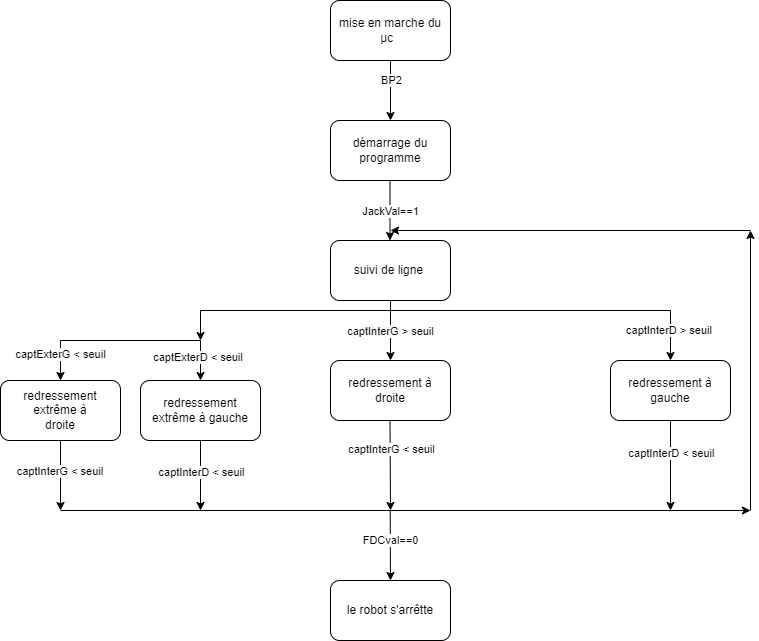
\includegraphics[width=1.2\linewidth]{img/mae/suivi ligne.png}}
  \captionof{figure}{\emph{Machine à états : suiveur de ligne.}}
  \label{fig:maesuiviligne}
\end{minipage}%
\end{figure}

Enfin, la fonction \emph{wait\_us(5000)} permet de définir un délai de 5 millisecondes entre chaque itération de la boucle de contrôle, ce qui permet d'éviter les erreurs de lecture des capteurs et de contrôler la vitesse du robot.

\subsubsection{Les options}
Dans ce projet nous avons eu la possibilité d’intégrer à nos codes des options nous rapportant des bonus, les 3 principales sont : 

\vfill
\noindent\makebox[\linewidth]{\rule{.8\paperwidth}{.6pt}}\\[0.2cm]
I.U.T. Nice Côte d'Azur - SAE Robot - 2023 \hfill goofyBot
\noindent\makebox[\linewidth]{\rule{.8\paperwidth}{.6pt}}
\newpage

\begin{itemize}
    \item Le raccourci : C’est une extension du programme suiveur de ligne, ce programme consiste en l’action de prendre un raccourci et donc automatiquement gagner du temps de parcours. Pour voir le raccourci, un bout de piste (ligne blanche) est placé 30cm en amont de la bifurcation, à gauche de la piste obligatoirement. Ce marqueur nous permet d’ordonner au robot de prendre le raccourci, et donc de tourner à gauche de 90°. Pour programmer le raccourci, en théorie d’abord,nous avons pensé créer une variable erreur gauche qui est égale a la tension du capteur extérieur gauche moins la tension du capteur intérieur droit. Il y en a une deuxième qui est la variable erreur droite qui prend pour valeur la tension du capteur extérieur droit moins la tension du capteur intérieur gauche. Ensuite, ces deux variables sont comparées et si le résultat de cette comparaison est supérieure à un seuil c’est qu' un marqueur a été repéré et donc qu'il va falloir tourner pour la piste de raccourci.

    \item Le stop-figure : Le stop figure est bonus de temps qui sera soustrait au temps final de suivi de ligne. Il consiste en l’arrêt du robot pendant le suivi de ligne ou après et la réalisation d’un tout du robot sur lui-même à 360°. Si il est réalisé pendant c’est un bonus de 10 secondes, et si il est après l’arrêt du robot, au fin de course, c’est 3 secondes de bonus. Pour coder celui-ci, théoriquement nous avons pensé utiliser un timer que l’on déclare avec la bibliothèque “time.h”, puis une variable tempsDebut et une autre tempsActuel. tempsDebut est affecté de la valeur de temps au début du programme et tempsActuel est  égale a tempsDebut et est en plus incrémentée en continu. Puis une simple comparaison avec une constante définie au début qui est en secondes pour savoir au bout de combien de temps on fait le stop Figure, nous envoie dans un état qui envoie aux bornes du moteur la même tension en sens inverse pendant le temps qu’il faut pour faire un tour. Une fois le tour fini, l’état redevient à celui du suivi.

    \item La priorité à droite : Celle- ci est moins importante, car n'apporte pas de bonus et nous ne l’avons pas faite, faute de temps. Cette option se résume à l'intégration d’un capteur supplémentaire sur le haut du robot tourné vers la droite et qui doit identifier qu’un robot arrive à droite et le laisse passer pendant le suivi de ligne.
\end{itemize}

\vfill
\noindent\makebox[\linewidth]{\rule{.8\paperwidth}{.6pt}}\\[0.2cm]
I.U.T. Nice Côte d'Azur - SAE Robot - 2023 \hfill goofyBot
\noindent\makebox[\linewidth]{\rule{.8\paperwidth}{.6pt}}
\newpage